\documentclass{article}
\usepackage[]{amsmath}
\usepackage{blindtext}
\usepackage[a4paper, total={7in, 9in}]{geometry}
\usepackage[]{hyperref}
\usepackage[noabbrev]{cleveref}
\usepackage[]{graphicx}


\title{Disturbance Response Planning with Trajectory Optimization}
\author{Trevor Long}


\begin{document}
\maketitle
\section{Introduction}

In this document I want to demonstrate the effectiveness of trajectory optimization and generating control strategies for aircraft subject to disturbances.
The intention for the present study is to demonstrate that this problem formulation provides reasonable results for relatively simple problems as proof-of-concept of the merit of this technqiue.
I will limit disucssion in this document to just the problem setup for the examples and the trajectory optimization formualtion at its highest level, a more detailed description of the formualtion itself will be written in the near future. 


\section{Problem Definition}\label{sec:problem-statement}

We wish to estimate what the 'best' control strategy is for an aircraft to maintain  a steady altitude whenich is subo an arbitrary gust field vertical gus, we will set up the problem as a search over the state space $\mathbf{x}(t), \mathbf{u}(t)$ over the time interval $t = [0, t_f]$ with start and end conditions which enforce the trimmed, level flight of the aircraft $\sum_{}^{}\mathbf{F}_b = 0$, $\sum\mathbf{M}_b = 0$, $\gamma = 0$. 
The problem is set up in discrete time so the interval $t = t_k$ for $ k= [1,2,...., N]$ and $t_k = k \cdot dt$ and all of the dynamics are represented as discrete values such that $\mathbf{x}(t),\mathbf{u}(t) \rightarrow \mathbf{x}[k],\mathbf{u}[k]$. \\
\\
As a desired outcome we will wish to minimize the deviation of the aircraft from the cruise altitude $z_c$. 
In the optimizer this desired outcome represented as the square error from the starting altitude $C(\mathbf{x}[k]) = \sum_{k=2}^{N} w_k \cdot(z_e[k] - z_e[k=1])^2$. 
This reperesents a hard constraint that might be encountered in a highly controlled airspace such as an a flight path through a city to a short landing field where the safe flight corridor is very small. \\
\\
To be precise about the formulation of the problem, I am using a collocation method to enforce the system dynamics between each discrete point the description of which is out of scope in this docuemnt. 
It is worth noting, however, that this means rather than a direct forward euler representation of the relationship between $x[k]$ and $x[k+1]$ a cubic polymial is used to constrain that relationship instead. \\
\\
I want to stress again that the purpose of this technique is to discover the \textit{best possible} response to a disturbance with perfect knowledge of the system and the disturbance. 
The trajectory optimization formulation allows the optimizer to consider not only how changes in $\mathbf{x}(t)$,$\mathbf{u}(t)$ propogate forward in time, but also backward since the trajectory is being solved across all-time using the dynamics as constraints rather than sequencially such as in an LQR controller. 
This formulation also allows for cost functions that are not linear combinations of $\mathbf{x}$ and $\mathbf{u}$ such as in LQR. 
The trajectory computed by the algorithim is globally optimal and can be seen as a benchmark as the \textit{best possible response} by which realizeable controllers constructed using other methods may be benchmarked for 'goodness'.
\section{Simulation Setup}

\subsection{Rigid Motion Model}
The motion of the aircraft is represented by a 2-dimensional point-mass model which has the freedom to move in the longitudinal plane with the state $\mathbf{x} $\ref{eq:state} and control of the throttle and elevator represented by $\mathbf{u}$ \ref{eq:control}; for simplicity the aircraft is assumed to rotate about the $\frac{1}{4}$ chord.
In the present model the body accelerations include only contributions from gravity, aerodynamics, and thrust forces which are computed and summed in the body frame.
Individual contributions from different surfaces are computed in the most natural frame (e.g. aerodynamicss in the wind frame) and trasnformed to the body frame for the summation using suitable rotation matrices.
\\
\begin{align} 
	\mathbf{x} &= \begin{Bmatrix}
		x_e,\; z_e,\; u_b,\; w_b,\; \theta,\; q
	\end{Bmatrix} \label{eq:state}\\
	\dot{\mathbf{x}} &= \begin{Bmatrix}
		u_e,\; w_e,\; a_{x,b},\; a_{z,b},\; q,\; \dot{q}
	\end{Bmatrix} \label{eq:deriv}\\
	\mathbf{u} &= \begin{Bmatrix}
		\delta_e,\; \delta_T \label{eq:control}
	\end{Bmatrix}
\end{align}
\\

\begin{align}
	\dot{u}_b &= \frac{1}{m}\sum F_x \label{eq:x-force-sum} = F_\mathrm{wing,x} + F_\mathrm{tail,x} + F_\mathrm{motor,x} + F_\mathrm{gravity,x}\\
	\dot{w}_b &= \frac{1}{m}\sum F_z \label{eq:z-force-sum} = F_\mathrm{wing,z} + F_\mathrm{tail,z} + F_\mathrm{motor,z} + F_\mathrm{gravity,z}\\
	\dot{u}_b &= \frac{1}{I_{yy}}\sum M_y \label{eq:y-mom-sum}	= M_\mathrm{wing} + M_\mathrm{tail} +  M_\mathrm{motor}
\end{align}
The dynamics of the controls in \cref{eq:control} are not directly modelled and are instead constrained by maximum rates described in \cref{sec:limits}. 
One reason to do this is to limit the size of the optimization problem which can get large very rapidly; the other is that at this point in the investigation I haven't looked in to directly modeling the control system dynamics. 
 
\subsection{Aerodyanmics and Thrust Models}

The aerodynamic forces on the point mass are computed using the sum of the contributions from the wing and the tail. The coefficients for the control surfaces are computed locally and scaled based on the area ratio of the wing and tail as shown in  \cref{eq:cl,eq:cd,eq:cm}. Forces and Moments are then computed by scaling the coefficeints using standard non-dimensionalization relationships.

\begin{align}
	c_L &= c_{\ell,\mathrm{wing}} + c_{\ell,\mathrm{tail}} \frac{S_\mathrm{tail}}{S_\mathrm{wing}} \label{eq:cl}\\
	c_D &= c_{D,\mathrm{wing}} + c_{D,\mathrm{tail}}\frac{S_\mathrm{tail}}{S_\mathrm{wing}} \label{eq:cd}\\
	c_M &= c_{M,\mathrm{wing}} + \left( c_{M,\mathrm{tail}} - c_{\ell,\mathrm{tail}} \ell_\mathrm{tail} \right) \frac{S_\mathrm{tail}}{S_\mathrm{wing}} \label{eq:cm}
\end{align}

For each airfoil the lift and pitching coefficients are calculated using linear theory for an airfoil with a hinged flap at angle $\delta_f$ at the location $\xi = 1-\frac{c_f}{c}$. The coefficients $A_0,A_1,A_2$ are functions of $\alpha$, $\delta_f$, and $\xi$. Drag is calcuated as the sum of a constant term and an induced quadratic term and so is a function of $c_\ell$, $AR$, $e$ for each surface.

\begin{align}
	c_\ell &= 2\pi (A_0 + 1/2*A_1) \\
	c_m &= -\pi/4*A_1 + A_2/4\\
	c_d &= c_{d0} + \frac{c_\ell^2}{\pi AR e}
\end{align}

The throttle model at present is currently computed as only a scaling of a given thrust-to-weight ratio $\frac{T}{mg}$ of 0.25. 
This scaling is multiplied by throttle position $\delta_T \in [0,1]$ to calcualte thrust force. 
This model does not account for loss as airspeed increases as would typically be observed, but is low enough so that the aircraft cannot accelerate to unconcstraiend speeds. \\

\subsection{Aircraft Parameters}

The physcial parameters of the model are based on those provided by students for the 821 surge aircraft and are presented in \cref{tbl:aircraft-params}. 
So far these parameters have provided reasonable results for the simulation and so are considered close enough to reality to be relied on. 

\begin{table}[!h]
	\centering
		\label{tbl:aircraft-params}
	\begin{tabular}{|c|c|}
		\hline
		\hline
		mass & 9.8 kg\\
		\hline
		Iyy & 2 kg-$\mathrm{m}^2$\\
		\hline
		S & 1.09$m^2$ \\
		\hline
		b & 3.05 m\\
		\hline
		$\mathrm{c}_ref$ & 0.38 m\\
		\hline
		$\mathrm{b}_\mathrm{tail}$ & 1.27 m\\
		\hline
		$\mathrm{c}_\mathrm{tail}$ & 0.25 m\\
		\hline
		$\mathrm{S}_\mathrm{tail}$ & $0.2 m^2$\\
		\hline 
		$\ell_\mathrm{tail}$ & 1 m  \\
		\hline
		\hline
	\end{tabular}

\end{table}

\subsection{General Limits on State and Control Terms} \label{sec:limits}
For solution stability and physical accuracy the problem formulation in the optimizer requires that upper and lower bounds be placed on all  $\mathbf{x}$ and $\mathbf{u}$ terms for all time. 
Some of these are 'soft' constraints on variables that are arbitrary but limit the solution space to something reasonable (such as the bounds on $x_e$ and $\theta$),  while others are set there to make certain responses 'reasonable' since some terms are not directly controlled by the plant physics such as the limits on the control rates$\delta_T$ and $\delta_e$. 
The limits shown in \cref{tbl:general-control-limits} are set for all simulations by default, but this does not restrict certain test cases may place more restrictive limits on $x$ and $u$ or combinations thereof if desired. 
\begin{table}[!h]
	\centering
	\caption{General upper and lower bounds on $\mathbf{x}$ and $\mathbf{u}$}
	\begin{tabular}{||c||c|c|c|}
		\hline
		term & lower limit & upper limit & unit\\
		\hline
		$x_e$ & 0 & 1e5 & m\\
		\hline
		$z_e$ & -1e5 & 0 &m\\
		\hline
		$u_b$ & 0 & 1e2& m/s\\
		\hline
		$w_b$ & 0 & 1e1 & m/s\\
		\hline
		$\theta$ & -360 & 360 & deg\\
		\hline
		$q$ & -20 & 20 & deg/s \\
		\hline
		$q$ & -20 & 20 & deg/s \\
		\hline
		$\delta_e$ & -15 & 15 & deg \\
		\hline
		$\delta_T$ & 0 & 1 & - \\ 
		\hline
		$\frac{d\delta_T}{dt}$ & -0.01 & 0.01 & -/sec \\ 
		\hline
		$\frac{d\delta_e}{dt}$ & -10 & 10 & deg/s \\ 
		\hline
	\end{tabular}
	\label{tbl:general-control-limits}
\end{table}
\subsection{Cruise Start and End Conditions}
The start and end constraints for cruise are pretty standard. 
The moment and force summations as well as the flight path angle are all enforced to be zero to hav ethe aircraft act as if it is in trimmed, level flight immediately before and after the disturbance. 


\begin{table}[!h]
	\centering
	\caption{Start and end constraints enforced for the cruise}\label{tbl:cruise-start-end-conditions}
	\begin{tabular}{| c |}
		\hline
		\hline 
		$V_\infty[0,N]$ = 15 m/s\\
		\hline
		$\theta^2[0,N]$ <= 36 \\
		\hline
		$\sum \mathbf{F}_b[0,N]$ == 0\\
		\hline
		$\sum \mathbf{M}_b[0,N]$ == 0\\
		\hline
		$\gamma_b[0,N]$ == 0\\
		\hline
		\hline
	\end{tabular}
\end{table}


\subsection{Gust Model} \label{sec:gust-model}
The wind gust at present is defined by a Gaussian function from  \cref{eq:gust-gaussian} and is intended to be representative only. 
This model approximates the shape of a thermal updraft but does not model things like mass conservation that would be present lin large air masses.
A real thermal updraft would almost certainly be accopmanied by a downdraft immediately before or after.  
\begin{equation}
	w_g(x) = w_{g,max} \exp{\left( -\frac{1}{2} \left(\frac{x-x_{center}}{\sigma}\right)^2\right)} \label{eq:gust-gaussian}
\end{equation}

\subsection{Cost Function}

As described in \cref{sec:problem-statement} the main cost function given to the optimizer for this investigation is the deviation from starting altitude. 
However, on discussion with Peter we also saw it necessary to add another summed cost which is the curvature of the control input $\mathbf{u}$.
The curvature in my notation here is given by the $curv(\cdot)$ function.\\
\\
The reason to add the additional curvature cost is to prevent the optimizer from settling on solutions which have very high-frequency inputs from the control surfaces which will tend to exploit either errors in $f(\mathbf{x},\mathbf{u})$ or the numerics of the problem more generally. 
The cost is given a very small weight of $1e^{-3}$ which is just enough to prevent the solution from being 'wiggly'. The equations that make up the cost function are shown in \cref{eq:altitude-cost,eq:curvature-cost,eq:total-cost}\\

\begin{align} 
	C_1(\mathbf{x}[k]) &= \sum_{k=2}^{N} w_k \cdot(z_e[k] - z_e[k=1])^2  \label{eq:altitude-cost}\\ 
	C_2(\mathbf{u}[k]) &= \sum_{k=1}^{N}{ \left(curv(\delta_e[k], t[k]) + curv(\delta_T[k], t[k]) \right) }\label{eq:curvature-cost}\\
	C(\mathbf{x},\mathbf{u}) &= C_1(\mathbf{x}) + C_2(\mathbf{u},t) \label{eq:total-cost}
	\end{align}


\subsection{Independent Axis} \label{sec:problem-grid}
The problem currently is set up to run with time as an independent variable from $[t_0, t_f] = [0,20]$ with a spacing $dt = 0.1s$ leading to a problem size of $N=200$.  
This definition does not represent a limitation on the problem formulation and any other variable could be chosen to parameterize the system. 
Additionally, it is possible in the present formulation to add $t_f$ and $dt$ as decision variables, though this has not currently been tested at length. 
These are most likely capabilties to look at moving forward.

\section{Results}
\subsection{Response to Thermal Updraft}
\begin{figure}
	\centering
	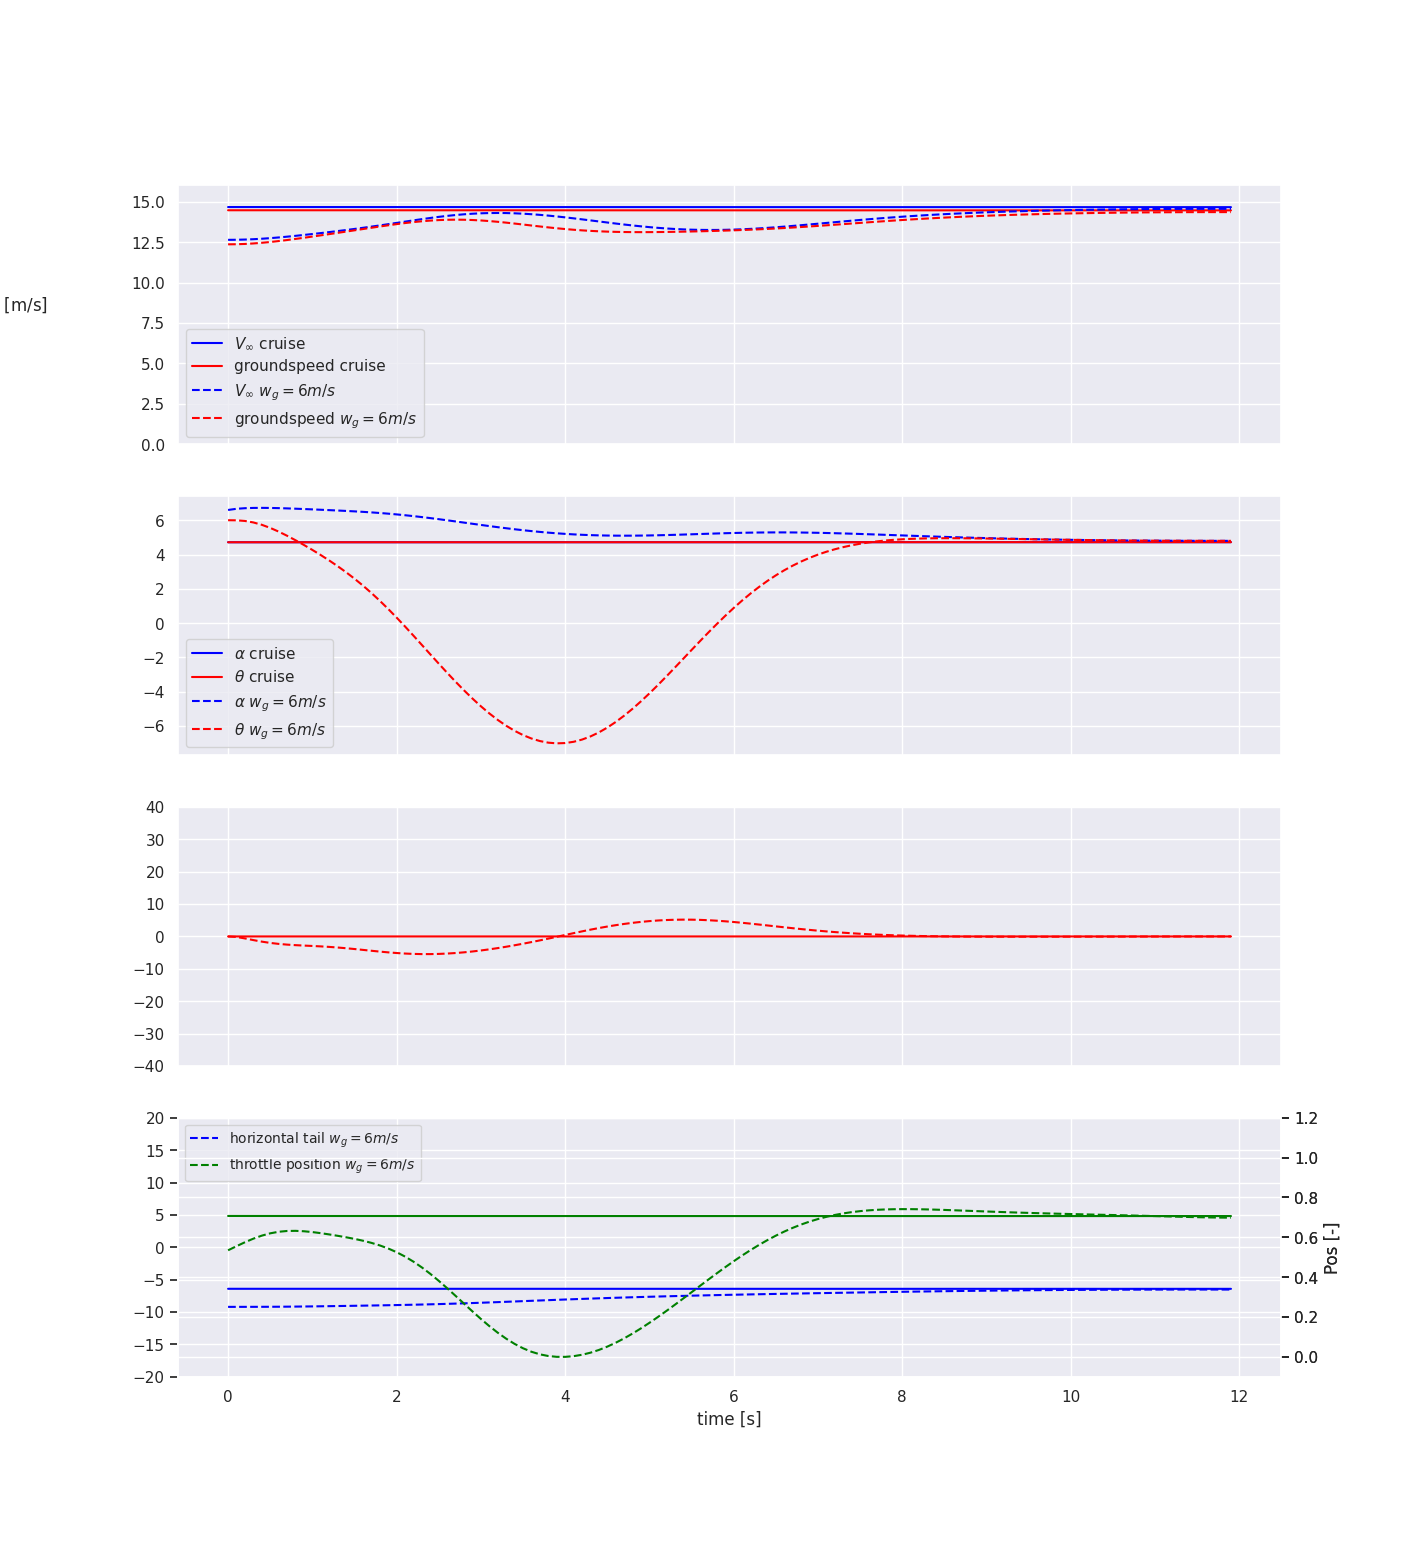
\includegraphics[width=0.8\textwidth]{time-trace-3ms.png}
	\caption{Time traces for select values for a updtraft with a core velocity of 3m/s (dashed) plotted against steady-cruise flight solution}
	\label{fig:cruise-3m/s gust}
\end{figure}
\begin{figure}
	\centering
	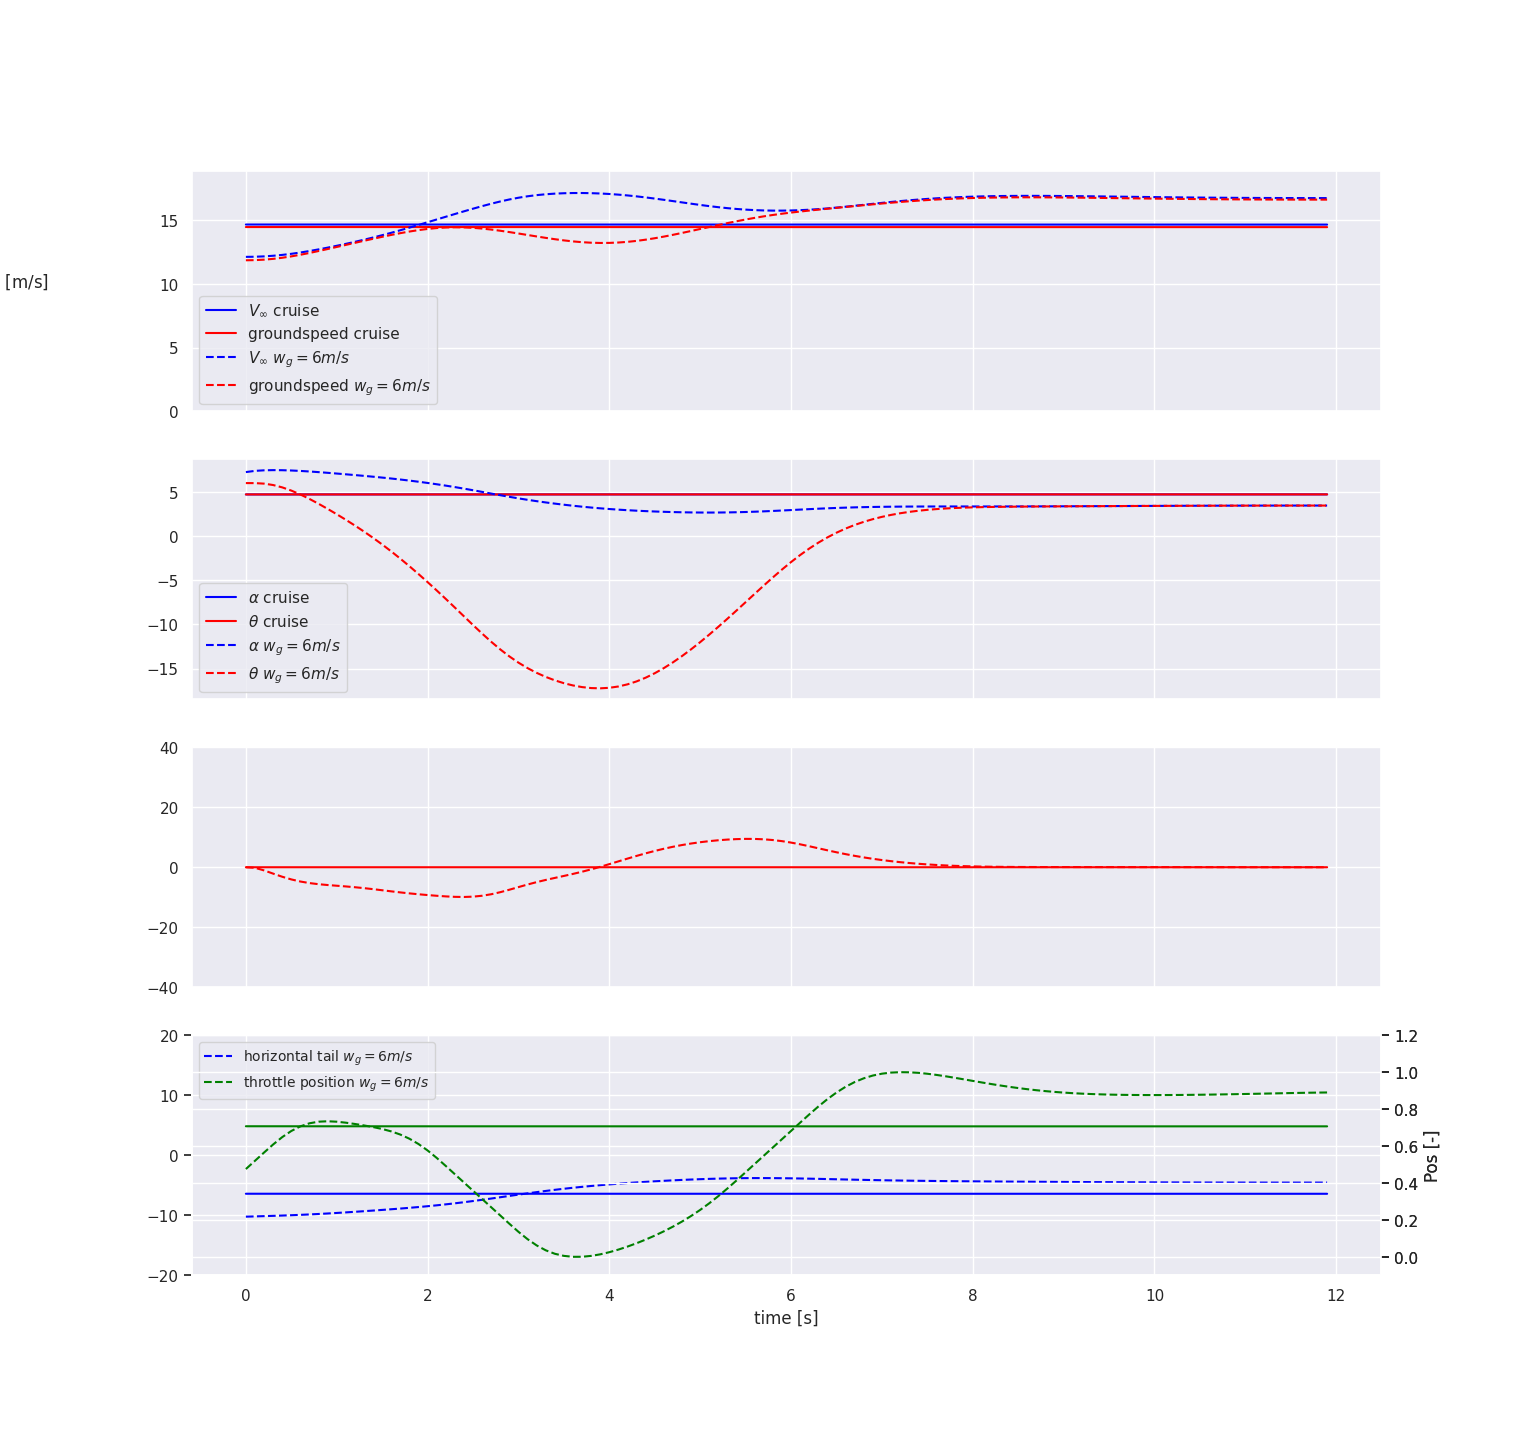
\includegraphics[width=0.8\textwidth]{time-trace-6ms.png}
	\caption{Time traces for select values for a updtraft with a core velocity of 3m/s (dashed) plotted against steady-cruise flight solution}
	\label{fig:cruise-6m/s gust}
\end{figure}

\section{Ongoing work}

\end{document}
